\label{chpt:results:characterisation of 12 new CVs} % for referencing this chapter elsewhere, use \ref{chpt:label}
\lhead{\emph{Eclipse modelling of 12 CVs}} % This is for the header on each page - perhaps a shortened title

% As previously mentioned, a primary focus of this thesis is to grow the population of eclipse modelled CVs.
A modest backlog of observed data was reduced, calibrated, and modelled, and the results are presented here. All CVs were fit using the new hierarchical model structure described in \S\ref{sect:modelling:optimising eclipse model parameters}, with eclipses binned together where possible, to reduce the complexity of the parameter space. Which specific data were binned together for each system, if any, is given in the tables in \S\ref{sect:observing:observation catalogue}.


\section{Systems chosen for modelling}

The systems modelled here were largely chosen based on their short periods, in an effort to uncover more period-bouncer CVs, as this population is under-sampled in previous eclipse-modelled CVs.
The systems chosen for modelling range in period from $1.4 - 2.2$ hours, and were drawn from a few sources.
The All-Sky Automated Survey for Supernovae (ASASSN) \citep{shappee2014} is sensitive to transients, and is a valuable tool to identify CVs by their outbursts for follow-up once they re-enter quiescence. Such systems are recognised by their ASASSN moniker.
% The vsnet alert system also provided several systems, which are marked below with (v).
The modelled systems in this thesis were:
\begin{itemize}
    \setlength\itemsep{0em}
    \item ASASSN-14hq
    \item ASASSN-14kb (a.k.a OGLE-LMC529.30.114)
    \item ASASSN-15pb
    \item ASASSN-17fo
    \item AY For (a.k.a H$\alpha$0242-2802) \citep{woudt2004}
    \item CSS090622 J215636+193242 (hereafter CSS090622) \citep{kato2012,thorstensen2016}
    \item CSS090102 J132536+210037 (hereafter CSS090102) \citep{kato2012}
    \item CSS090419 J162620-125557 (hereafter CSS090419) \citep{kato2012}
    \item MASTER OT J001400.25-561735.0 (hereafter MAS0014) (Woudt, private communication)
    \item OGLE BLG-ECL-000082 (a.k.a BLG510.16.126296, hereafter OGLE82)
    \item SDSS J074859.6+312512.7 (hereafter SDSS J0748) \citep{kato2016}
    \item SDSS J152419.33+220920.0 (hereafter SDSS J1524) \citep{southworth2010,michel2013}
\end{itemize}

ASASSN-14hq and ASASSN-15pb was observed by \citet{paterson2019}, though note that the observations used in this thesis pre-date this publication. These two systems were noted to be in outburst, as of late 2014 in the case if ASASSN-14hq, and 2015 in the case of ASASSN-15pb.

AY For had the white dwarf and donor stars' masses estimated spectroscopically in \citet{mason2005} to be $M_{\rm wd} \sim 0.64 M_\odot$ and $M_{\rm donor} \sim 0.17 M_\odot$, with no error reported. This measurement, however, is dubious. It is based on inferring a donor mass and radius from the period using the model $M_{\rm donor} - P$ relation presented in \citet{howell2002}. This is then used to calculate a white dwarf mass. AY For is also claimed by \citet{mason2005} to be a pre-period minimum system.


\section{Results}

All eclipses presented are well-described by their fits, with small residuals. The lightcurves are contained in Appendix~\ref{appendix:lightcurves}, along with the white dwarf flux distributions compared to the cooling tracks, in Appendix~\ref{appendix:white dwarf fluxes}. The example system of ASASSN-14kb has the lightcurve and flux distribution is shown in Figure~\ref{fig:results:12 new CVs:ASASSN-14kb all lightcurves}, and Figure~\ref{fig:results:12 new CVs:ASASSN-14kb flux plot}, respectively.
In a few cases, the GP appears as a flat line along a residual of 0, despite some obvious scatter, for example in ASASSN-14hq, seen in Figure~\ref{fig:ASASSN-14hq all lightcurves cont}. This is expected, as in these cases the residuals are fully described by the error in flux and the GP likelihood becomes dominated by the priors, sampling small values of GP amplitude.

\begin{figure}
    \centering
    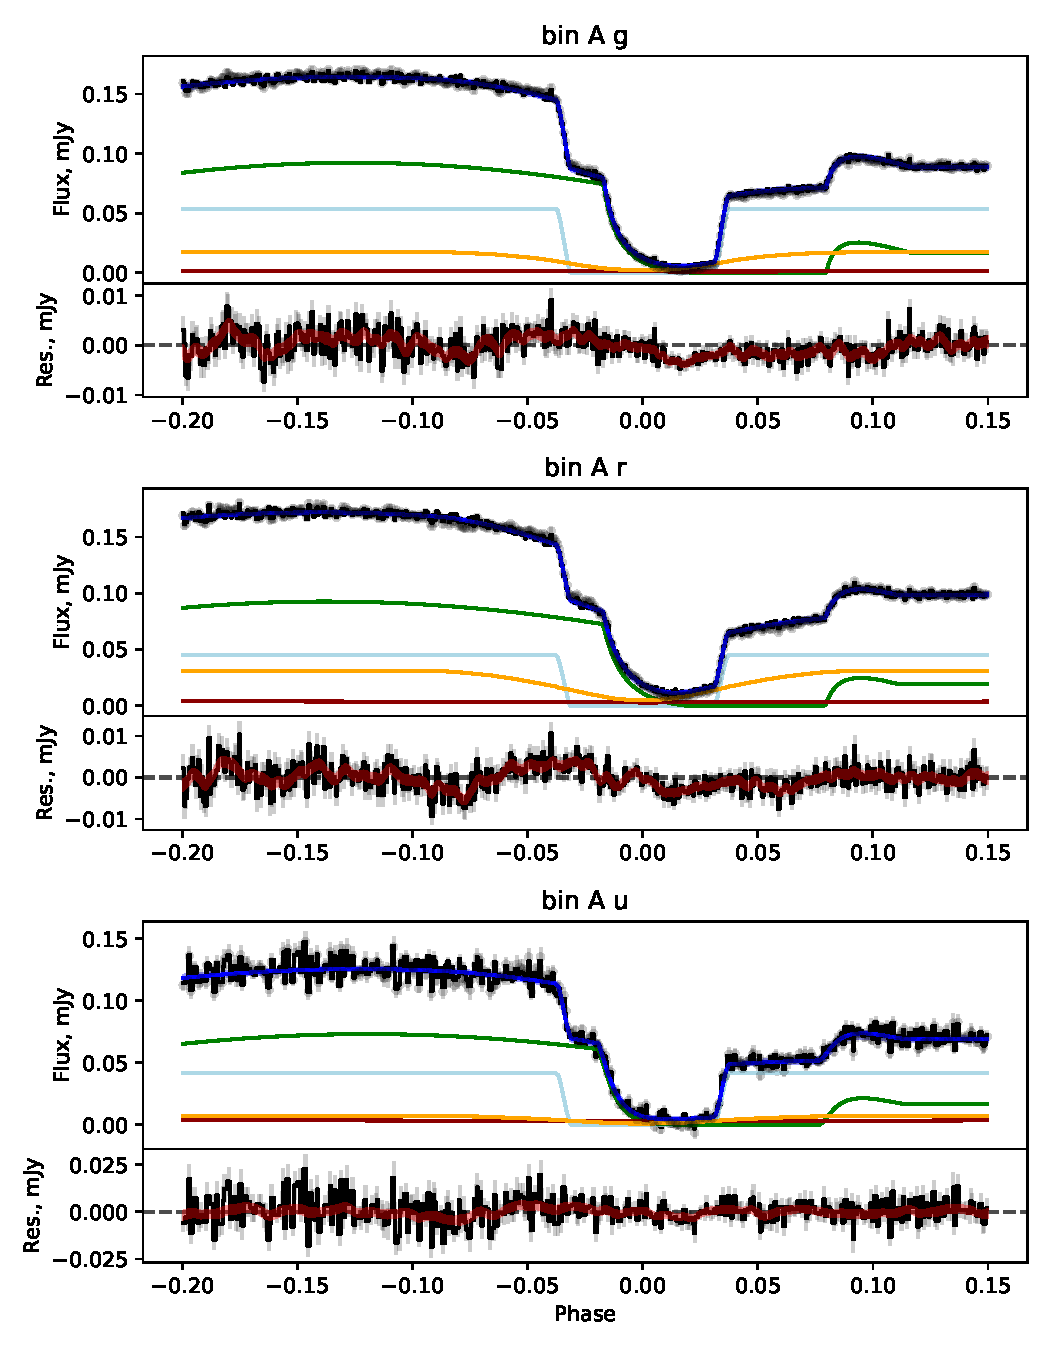
\includegraphics[width=\textwidth]{figures/results/ASASSN-14kb/ASASSN-14kb_ex_1.pdf}
    \caption{ASASSN-14kb lightcurve models. {\it Top}:~{\bf grey points} are the observed flux, and note that the photometric system is the SDSS as per \S\ref{sect:observations:flux calibrating the lightcurve}; {\bf black line} is the observed flux, with the mean Gaussian process sample subtracted; the {\bf dark blue line} is the mean lightcurve model, and the {\bf blue band} is the standard deviation on this in the MCMC chain. The components of the model are also shown: the {\bf light blue line} is the white dwarf flux, {\bf green line} is the bright spot, {\bf orange line} is the disc, and the {\bf red line} is the donor. {\it Bottom}:~The residuals between the data and model are plotted as the {\bf black line}, with grey error bars. The Gaussian process 1-sigma region is shown as a {\bf red band}.}
    \label{fig:results:12 new CVs:ASASSN-14kb all lightcurves}
\end{figure}
\begin{figure}
    \centering
    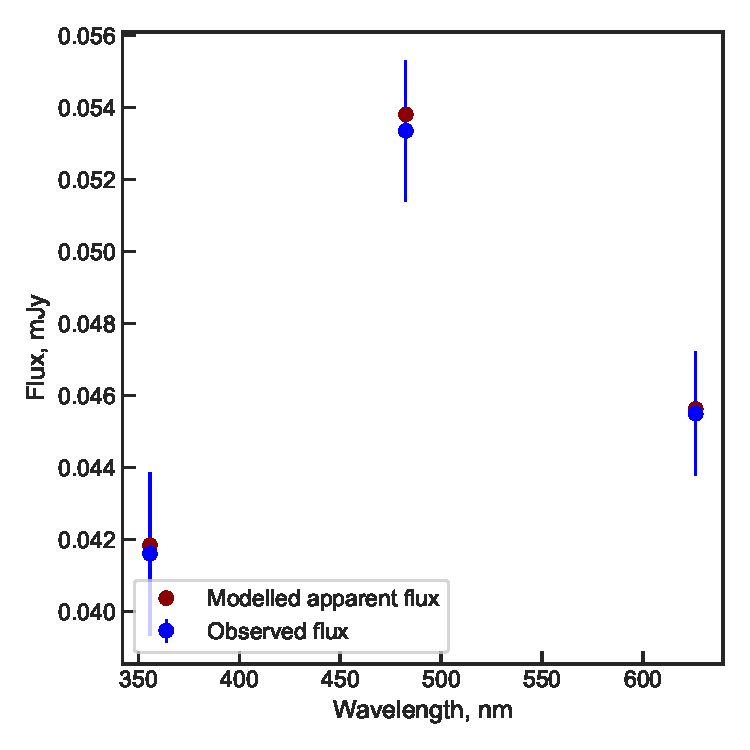
\includegraphics[width=\textwidth]{figures/results/ASASSN-14kb/fluxplot.pdf}
    \caption{ASASSN-14kb observed white dwarf fluxes, compared to the best-fit model atmosphere.}
    \label{fig:results:12 new CVs:ASASSN-14kb flux plot}
\end{figure}

The white dwarf fluxes of AY For were not well-described by the white dwarf cooling tracks, similarly to the systems in \S\ref{sect:three white dwarfs:method WD atmosphere fits}. This is likely to be a real effect, as the field about AY For was observed by the PANSTARRS survey, and the comparison star SDSS magnitudes are reported. The flux calibration performed as standard with ULTRACAM is within 2\% of the PANSTARRS values.
In addition, the white dwarf fluxes of CSS090419 and CSS090622 appear to significantly brighten in the $i'$ band, seen in Figure~\ref{fig:CSS090419 flux plot} and Figure~\ref{fig:CSS090622 flux plot}, which cannot be described by the white dwarf models used here. However, the disagreement in each case is well within $2 \sigma$, and not seen in the other $i$ band observation, ASASSN-15pb, suggesting this is not a systematic issue. For both systems, the characterisation can still be considered robust.

Table~\ref{table:12 new cvs:system_parameters} details the physical parameters of these 12 new systems.

\newpage

\begin{landscape}

    \begin{table*}
        \centering
        \caption{The system parameters found for the CVs analysed here. The reported $\pi$ is the posterior distribution from fitting the white dwarf fluxes, c.f. \S\ref{sect:modelling:fitting white dwarf colours}.}
        \label{table:12 new cvs:system_parameters}
        \begin{tabular}{cccccc}
            \hline \\
            \textbf{System Name:}      & \textbf{ASASSN-14hq}    & \textbf{ASASSN-14kb}     & \textbf{ASASSN-15pb}      & \textbf{ASASSN-17fo}      & \textbf{AY For}       \\
            \hline \hline \\
            $M_\mathrm{WD}/M_\odot$    & $0.67\pm0.01$           & $0.74\pm0.02$            & $0.72\pm0.03$             & $0.85\pm0.01$             & $0.78\pm0.02$         \\
            $R_\mathrm{WD}/R_\odot$    & $0.0119\pm0.0001$       & $0.0113\pm0.0002$        & $0.0115\pm0.0005$         & $0.0099\pm0.0001$         & $0.0106\pm0.0003$ \\
            $M_\mathrm{donor}/M_\odot$ & $0.097\pm0.002$         & $0.134\pm0.003$          & $0.148\pm0.008$           & $0.109\pm0.002$           & $0.106\pm0.006$ \\
            $R_\mathrm{donor}/R_\odot$ & $0.157\pm0.001$         & $0.164\pm0.001$          & $0.210\pm0.004$           & $0.1436\pm0.0007$         & $0.162\pm0.003$ \\
            $q$                        & $0.145\pm0.002$         & $0.182\pm0.002$          & $0.206\pm0.004$           & $0.1267\pm0.0005$         & $0.136\pm0.004$ \\
            \hline
            $P$, hours                 & $1.78384800(7)$         & $1.63453(1)$             & $2.23896(3)$              & $1.477147(2)$             & $1.790756(1)$ \\
            $a/R_\odot$,               & $0.681\pm0.004$         & $0.670\pm0.005$          & $0.824\pm0.014$           & $0.646\pm0.003$           & $0.717\pm0.007$ \\
            $i$                        & $80.35\pm0.06$          & $84.4\pm0.1$             & $79.4\pm0.1$              & $84.23\pm0.03$            & $84.0\pm0.2$ \\
            $K_\mathrm{WD}$, km/s      & $58.0\pm0.9$            & $76.2\pm1$               & $75\pm2$                  & $60.2\pm0.4$              & $57.8\pm2.0$ \\
            $K_\mathrm{donor}$, km/s   & $399\pm2$               & $419\pm3$                & $364\pm6$                 & $468\pm2$                 & $425\pm4$ \\
            \hline
            $\pi$, mas                 & $3.40\pm0.07$           & $2.78\pm0.11$            & $1.0\pm0.2$               & $1.79\pm0.36$             & $2.12\pm0.16$ \\
            $T_{\rm eff}$, K           & $14819\pm800$           & $17700\pm1000$           & $19200\pm1600$            & $14800\pm600$             & $18100\pm500$ \\
            $\log(g), {\rm cgs}$       & $8.11\pm0.02$           & $8.21\pm0.03$            & $8.17\pm0.06$             & $8.37\pm0.02$             & $8.28\pm0.04$ \\
            \hline
            \hline
        \end{tabular}
    \end{table*}

    \begin{table*}
        \centering
        \caption{Table~\ref{table:12 new cvs:system_parameters}, continued.}
        \label{table:12 new cvs:system_parameters cont 1}
        \begin{tabular}{cccccc}
            \hline \\
            \textbf{System Name:}      & \textbf{CSS090102}     & \textbf{CSS090419}    & \textbf{CSS090622}    & \textbf{OGLE82}   & \textbf{SDSS J0748} \\
            \hline \hline \\
            $M_\mathrm{WD}/M_\odot$    & $0.62\pm0.03$          & $0.59\pm0.08$         & $0.67\pm0.06$         & $0.83\pm0.01$     & $0.68\pm0.02$ \\
            $R_\mathrm{WD}/R_\odot$    & $0.0126\pm0.0004$      & $0.0122\pm0.0009$     & $0.0112\pm0.0007$     & $0.0099\pm0.0002$ & $0.0121\pm0.0004$ \\
            $M_\mathrm{donor}/M_\odot$ & $0.060\pm0.003$        & $0.087\pm0.011$       & $0.104\pm0.009$       & $0.131\pm0.004$   & $0.066\pm0.004$ \\
            $R_\mathrm{donor}/R_\odot$ & $0.119\pm0.002$        & $0.152\pm0.007$       & $0.155\pm0.005$       & $0.170\pm0.002$   & $0.117\pm0.002$ \\
            $q$                        & $0.094\pm0.002$        & $0.146\pm0.003$       & $0.159\pm0.008$       & $0.157\pm0.002$   & $0.095\pm0.004$ \\
            \hline
            $P$, hours                 & $1.49723786(5)$        & $1.81062621(6)$       & $1.702302(6)$         & $1.7263398(6)$    & $1.39947(1)$ \\
            $a/R_\odot$,               & $0.582\pm0.008$        & $0.660\pm0.030$       & $0.661\pm0.020$       & $0.720\pm0.006$   & $0.575\pm0.007$ \\
            $i$                        & $88.7\pm0.6$           & $80.9\pm0.1$          & $88.2\pm0.6$          & $83.9\pm0.1$      & $81.7\pm0.2$ \\
            $K_\mathrm{WD}$, km/s      & $40.9\pm1.2$           & $56.0\pm2.7$          & $63.7\pm2.5$          & $68.5\pm1.0$      & $42.2\pm1.8$ \\
            $K_\mathrm{donor}$, km/s   & $431\pm6$              & $381\pm16$            & $408\pm12$            & $435\pm3$         & $450\pm5$ \\
            \hline
            $\pi$, mas                 & $1.41\pm0.30$          & $1.42\pm0.69$         & $2.02\pm0.27$         & $3.82\pm0.12$     & $1.83\pm0.14$ \\
            $T_{\rm eff}$, K           & $14800\pm1200$         & $18200\pm9000$        & $9800\pm1500$         & $18000\pm4000$    & $22500\pm3000$ \\
            $\log(g), {\rm cgs}$       & $8.00\pm0.33$          & $8.04\pm0.12$         & $8.16\pm0.08$         & $8.37\pm0.03$     & $8.11\pm0.03$ \\
            \hline
            \hline
        \end{tabular}
    \end{table*}

    \begin{table*}
        \centering
        \caption{Table~\ref{table:12 new cvs:system_parameters}, continued.}
        \label{table:12 new cvs:system_parameters cont 2}
        \begin{tabular}{ccc}
            \hline \\
            \textbf{System Name:}      & \textbf{MASOT0014}     & \textbf{SDSS J1524} \\
            \hline \hline \\
            $M_\mathrm{WD}/M_\odot$    & $0.86\pm0.03$          & $ $ \\
            $R_\mathrm{WD}/R_\odot$    & $0.0097\pm0.0003$      & $ $ \\
            $M_\mathrm{donor}/M_\odot$ & $0.122\pm0.007$        & $ $ \\
            $R_\mathrm{donor}/R_\odot$ & $0.165\pm0.003$        & $ $ \\
            $q$                        & $0.142\pm0.004$        & $ $ \\
            \hline
            $P$, hours                 & $1.7167077(5)$         & $ $ \\
            $a/R_\odot$,               & $0.722\pm0.008$        & $ $ \\
            $i$                        & $84.8\pm0.3$           & $ $ \\
            $K_\mathrm{WD}$, km/s      & $63.2\pm2$             & $ $ \\
            $K_\mathrm{donor}$, km/s   & $445\pm5$              & $ $ \\
            \hline
            $\pi$, mas                 & $2.42\pm0.11$          & $ $ \\
            $T_{\rm eff}$, K           & $17300\pm1000$         & $ $ \\
            $\log(g), {\rm cgs}$       & $8.37\pm0.04$          & $ $ \\
            \hline
            \hline
        \end{tabular}
    \end{table*}
\end{landscape}

\todo{Add SDSS J1524}